\newpage
\addcontentsline{toc}{section}{IP Specification}
\section*{\hfill IP Specification}

\subsection*{\fontsize{14}{16}\selectfont Overview}
\addcontentsline{toc}{subsection}{Overview}
The figure \ref{fig:ocla1} presents a detailed internal block diagram of the OCLA (On-Chip Logic Analyzer). It is characterized by a modular design, comprising various modules such as the OCLA AXI-lite Slave interface, Trigger Control Unit, Sampler Buffer, OCLA Controller, and OCLA On-Chip Trace Memory modules. Furthermore, it is designed as a multi-clock system, with a sampling clock and an AXI bus clock.
\\ \\The sampling clock is synchronized with the clock of the System/Design under test (S/DUT) and is used to sample data on the rising edge of this clock, based on the configured sampling mode of the OCLA. 
\\ \\The OCLA can be configured through the AXI interface on the rising edge of the AXI bus clock. The collected data can be read via the AXI interface, also running on the AXI clock.
\\ \\The modules that control the sampling operation of the OCLA, such as the Sampler Buffer and the OCLA Controller, operate on the sampling clock. In contrast, the AXI Slave and the Stream Out Buffer modules operate on the AXI clock and are used to configure or read the acquired data from the trace memory.
\\ \\The On-Chip trace memory controller is implemented as a circular buffer based on a modified asynchronous FIFO. This design handles the clock domain crossing of the trace memory data and configuration data, ensuring efficient and accurate data transfer between the different modules.

\begin{figure}[h]\centering % Using \begin{figure*} makes the figure take up the entire width of the page
	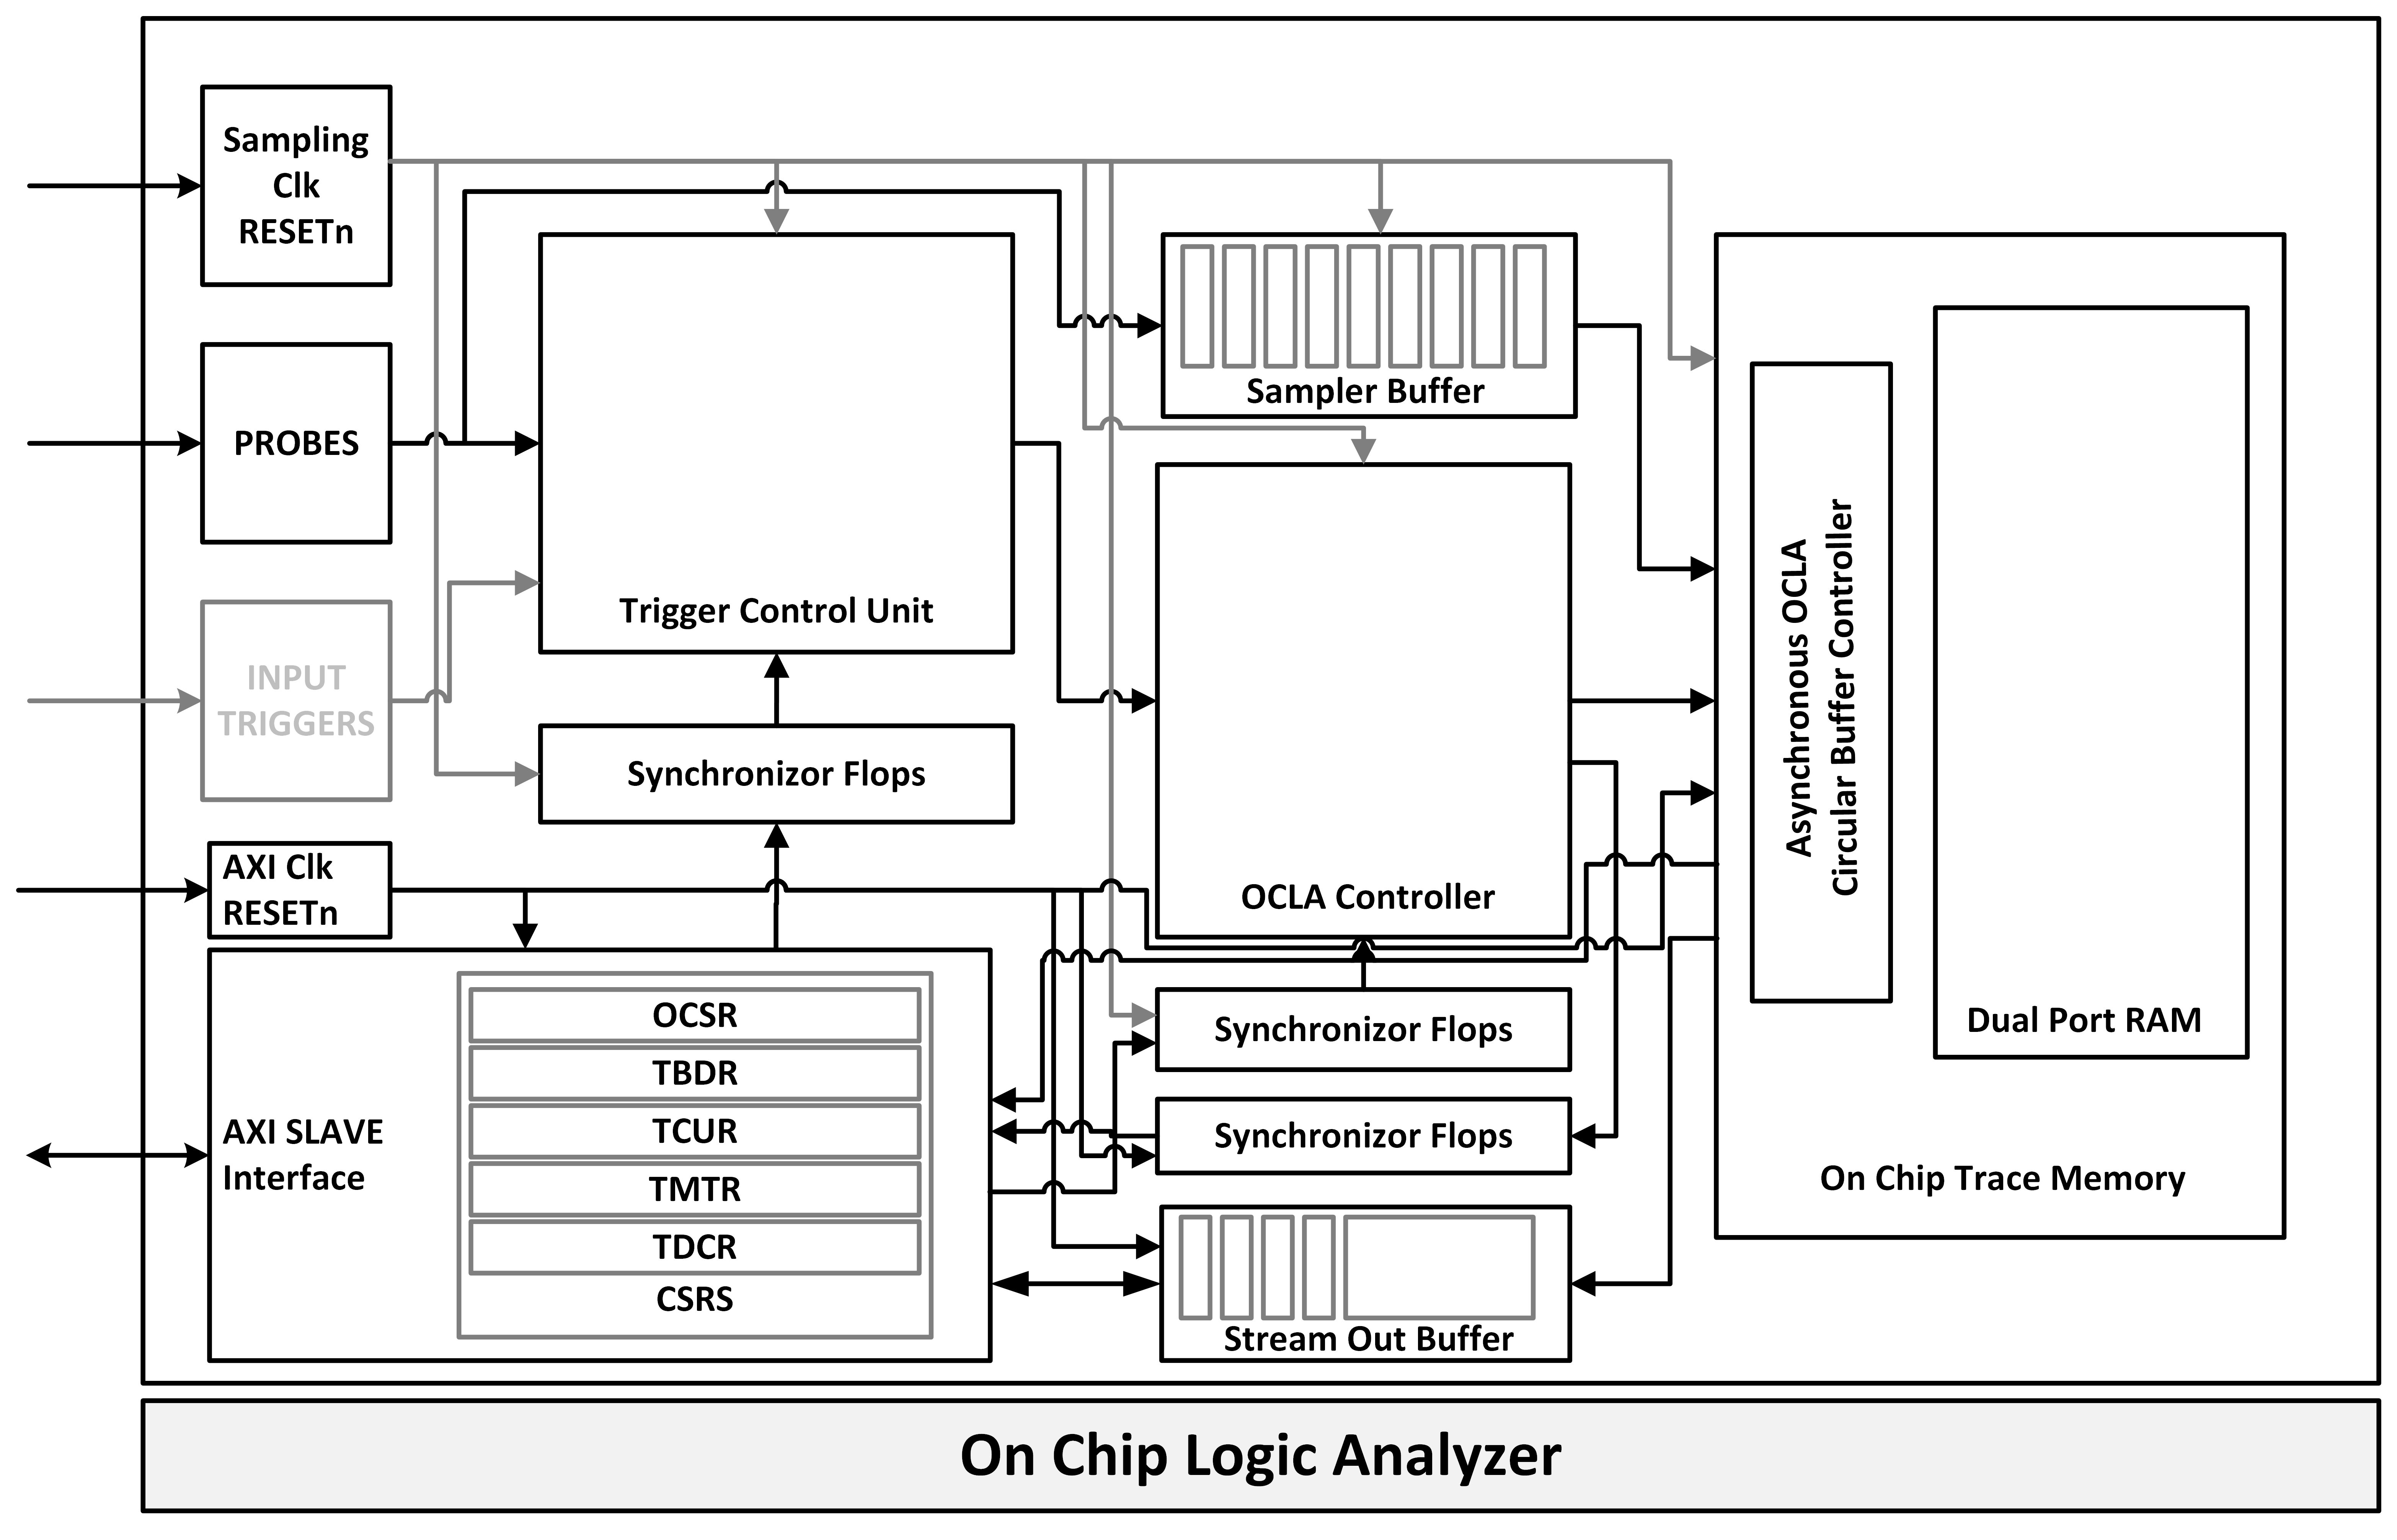
\includegraphics[width=\linewidth]{ocla1}
	\caption{Top Module}
	\label{fig:ocla1}
\end{figure}


\subsection*{\fontsize{14}{16}\selectfont Trigger}
The OCLA IP core utilizes a trigger mechanism to initiate the capture of probe data samples. The trigger signal can be selected from a variety of sources, including probe input signals or trigger input signals. 
\\OCLA also allows for the configuration of various trigger conditions on the trigger signal, such as level, edge, and value compare. The OCLA continually monitors the trigger signal, and data sampling begins when all of the trigger conditions in the active trigger pattern are satisfied. 
\\Additionally, the OCLA features a user-configurable trigger mode setting, which determines the amount of data that should be acquired by the system prior to and following the trigger event. The acquired data is stored in a circular buffer for further analysis, which enables the system to efficiently handle large data sets and continuously update the data being captured.
\\ \\OCLA supports simple and advance trigger options.

\begin{itemize}[noitemsep]
	\item \textbf{Simple Trigger Mode}: The trigger condition is applied on a single probe channel.
	\item \textbf{Advance Trigger Mode}: The trigger condition is be applied on two probe channels with boolean comparison. 
\end{itemize}
\subsection*{\fontsize{14}{16}\selectfont Trigger Conditions}
Multiple options for trigger conditions are available for probe and input triggers signals. Following lists the trigger conditions:
\begin{longtable}{|l|l|}
	\hline
	\textbf{Trigger Condition} & \textbf{Description}                                                                                                \\ \hline
	\endfirsthead
	%
	\endhead
	%
	Don’t Care                 & Default trigger condition. The channel is not \\ & used to determine the trigger event.                                  \\ \hline
	Low level                  & OCLA triggers when the probe channel is low.                                                                              \\ \hline
	High level                 & OCLA triggers when the probe channel is high.                                                                             \\ \hline
	Falling Edge               & OCLA triggers on the falling edge the probe channel.                                                                          \\ \hline
	Rising Egde                & OCLA triggers on the falling edge the probe channel.                                                                           \\ \hline
	Either Edge                & OCLA triggers on either edge of the probe channel.                                                                \\ \hline
	Value Comparison           & OCLA triggers when the value of a probe channel is \\ & equal /less than / greator than some user specified value.       \\ \hline

	Boolean Trigger equations  & \begin{tabular}[c]{@{}l@{}}Advance Trigger Conditions AND, OR, \\  \textless{}, \textgreater{}, == etc\end{tabular} \\ \hline
	\caption{Trigger Conditions}
	\label{tab:Trigger-Condition}                                                                                                                    \\
\end{longtable}
\subsection*{\fontsize{14}{16}\selectfont Trigger Modes}
The common trigger modes are post trig, pre trig, center and countinous.
\begin{itemize}[noitemsep]
	\item \textbf{Pre triggered} the
	      stored data set will consist of data sampled after the trigger.
	\item \textbf{Post triggered} is the opposite and in
	      this mode the logic analyzer stops the sampling immediately when the trigger is raised
	      thus only storing data from before the triggering event.
	\item \textbf{Center triggered} is a combination putting the
	      triggering event in the middle of the sampled data set
	\item \textbf{Continous trigger} mode continounsly samples data.
\end{itemize}

\subsection*{Fix number of samples}
The OCLA IP core can be configured to dynamically sample a specified number of probe samples, rather than utilizing the default trace memory depth, at runtime. 
This allows for greater flexibility in the debuging process, as the number of probe samples can be adjusted to suit the specific requirements of runtimme debuging.
\subsection*{\fontsize{14}{16}\selectfont Standards}
\addcontentsline{toc}{subsection}{Standards}
The AXI4-Lite Slave interface is compliant with the AMBA® AXI Protocol
Specification.
\par\noindent\rule{\textwidth}{0.4pt}
  % \lipsum
\newpage
  \subsection*{\fontsize{14}{16}\selectfont IP Support Details}
  \addcontentsline{toc}{subsection}{IP Support Details}
  The table  \ref{tab:ip_sup_tab} presents the specifics of IP support for the OCLA IP Core, including pertinent information such as synthesis, simulation and source details.
% Please add the following required packages to your document preamble:
% \usepackage{longtable}
% Note: It may be necessary to compile the document several times to get a multi-page table to line up properly
% Please add the following required packages to your document preamble:
% \usepackage{longtable}
% Note: It may be necessary to compile the document several times to get a multi-page table to line up properly
\\ \\


\noindent\begin{minipage}{\linewidth}
	\resizebox{\linewidth}{!}{%
	\begin{tabular}{|>{\hspace{0pt}}m{0.063\linewidth}|>{\hspace{0pt}}m{0.067\linewidth}|>{\hspace{0pt}}m{0.094\linewidth}|>{\hspace{0pt}}m{0.1\linewidth}|>{\hspace{0pt}}m{0.075\linewidth}|>{\hspace{0pt}}m{0.117\linewidth}|>{\hspace{0pt}}m{0.106\linewidth}|>{\hspace{0pt}}m{0.15\linewidth}|>{\hspace{0pt}}m{0.083\linewidth}|>{\hspace{0pt}}m{0.075\linewidth}|} 
	\hline
	\multicolumn{2}{|>{\hspace{0pt}}m{0.13\linewidth}|}{\textbf{Compliance}} & \multicolumn{5}{>{\centering\hspace{0pt}}m{0.492\linewidth}|}{\textbf{IP Resources}}                                         & \multicolumn{3}{>{\centering\arraybackslash\hspace{0pt}}m{0.308\linewidth}|}{\textbf{Tool Flow}}  \\ 
	\hline
	\textbf{Device} & \textbf{Interface}                                               & \textbf{Source Files} & \textbf{Constraint File} & \textbf{Testbench} & \textbf{Simulation Model} & \textbf{Software Driver} & \textbf{Analyze and Elaboration} & \textbf{Simulation} & \textbf{Synthesis}                       \\ 
	\hline
	GEMINI          & AXI4-lite                                                        & Systemverilog         & SDC                      & -                  & -                         & -                        & Raptor                           & Third Party         & Raptor                                   \\
	\hline
	\end{tabular}
	}
	\centering
	\captionof{table}{IP Information}
	\label{tab:ip_sup_tab}
	\end{minipage}

\subsection*{\fontsize{14}{16}\selectfont Resource Utilization}
\addcontentsline{toc}{subsection}{Resource Utilization}
% Please add the following required packages to your document preamble:
% \usepackage{multirow}
% \usepackage{graphicx}
% Please add the following required packages to your document preamble:
% \usepackage{multirow}
% \usepackage{longtable}
% Note: It may be necessary to compile the document several times to get a multi-page table to line up properly
The table \ref{tab:ip_ru} presents the resources utilization of OCLA IP for the Gemini device within the Raptor Design Suite, specifically detailing the statistics of resource utilization for both the minimum and maximum configurations of the OCLA.
\\ \\
\noindent\begin{minipage}{\linewidth}
	\resizebox{\linewidth}{!}{%
	\begin{tabular}{|l|l|l|l|l|} 
	\hline
	\multicolumn{2}{|c|}{\textbf{Configuration}}              & \multicolumn{3}{c|}{\textbf{Resource Utillization}}             \\ 
	\hline
	\multirow{6}{*}{Minimum Resource} & Options               & Configuration & Resources              & Utillized              \\ 
	\cline{2-5}
									  & Number of Probe       & 1             & LUT                    & 263                    \\ 
	\cline{2-5}
									  & Trace Memory Depth    & 32            & \multirow{2}{*}{FLOPS} & \multirow{2}{*}{138}   \\ 
	\cline{2-3}
									  & Advance Trigger Mode  & OFF           &                        &                        \\ 
	\cline{2-5}
									  & Value Compare Feature & OFF           & BRAM                   & 1                      \\ 
	\cline{2-5}
									  & Input Triggers        & 0             & DSP                    & 0                      \\ 
	\hline
	\multirow{6}{*}{Maximum Resource} & Options               & Configuration & Resources              & Utillized              \\ 
	\cline{2-5}
									  & Number of Probe       & 1024          & LUT                    & 1068                   \\ 
	\cline{2-5}
									  & Trace Memory Depth    & 1024          & \multirow{2}{*}{FLOPS} & \multirow{2}{*}{5466}  \\ 
	\cline{2-3}
									  & Advance Trigger Mode  & ON            &                        &                        \\ 
	\cline{2-5}
									  & Value Compare Feature & ON            & BRAM                   & 29                     \\ 
	\cline{2-5}
									  & Input Triggers        & 32            & DSP                    & 0                      \\
	\hline
	\end{tabular}
	}
	\centering
	\captionof{table}{Resource Utillization}	
	\label{tab:ip_ru}
	\end{minipage}
  % \lipsum
  \newpage
\subsection*{\fontsize{14}{16}\selectfont Ports}
\addcontentsline{toc}{subsection}{Port List}

Table \ref{tab:ocla-intr} lists the top interface ports of the OCLA.

% \usepackage{array}
% \usepackage{longtable}
% \usepackage{colortbl}


  
\begin{longtable}{|>{\hspace{0pt}}m{0.292\linewidth}|>{\centering\hspace{0pt}}m{0.056\linewidth}|>{\hspace{0pt}}m{0.585\linewidth}|} 
\hline
 \multicolumn{1}{|>{\hspace{0pt}}m{0.292\linewidth}|}{\textbf{  {Signal Name}}} & \textbf{  {I/O}} & \multicolumn{1}{>{\centering\arraybackslash\hspace{0pt}}m{0.585\linewidth}|}{\textbf{  {Description}}} \endfirsthead
 \hline
 \multicolumn{3}{|>{\hspace{0pt}}m{0.932\linewidth}|}{\textbf{Sampling Clock and Reset }} \\ 
\hline
i\_sample\_clk & I & Clock to Sample the Probe Data.\par{}It must be same as the Design under test \\ 
\hline
i\_rstn & I & Reset port of OCLA and it must be same\par{}~as design under test \\ 
\hline
\multicolumn{3}{|>{\hspace{0pt}}m{0.932\linewidth}|}{\textbf{AXI Clock and Reset }} \\ 
\hline
i\_S\_AXI\_ACLK & I & AXI4-Lite Clock \\ 
\hline
i\_S\_AXI\_ARESETN & I & AXI4-Lite RESET \\ 
\hline
\multicolumn{3}{|>{\hspace{0pt}}m{0.932\linewidth}|}{\textbf{AXI WRITE ADDRESS CHANNEL }} \\ 
\hline
s\_axil\_awvalid & I & AXI4-Lite Write address valid \\ 
\hline
s\_axil\_awready & O & AXI4-Lite Write address ready \\ 
\hline
s\_axil\_awaddr & I & AXI4-Lite Write address \\ 
\hline
s\_axil\_awprot & I & AXI4-Lite Protection type \\ 
\hline
\multicolumn{3}{|>{\hspace{0pt}}m{0.932\linewidth}|}{\textbf{AXI WRITE DATA CHANNEL }} \\ 
\hline
s\_axil\_wvalid & I & AXI4-Lite Write valid \\ 
\hline
s\_axil\_wready & O & AXI4-Lite Write ready. \\ 
\hline
s\_axil\_wdata & I & AXI4-Lite Write data \\ 
\hline
s\_axil\_wstrb & I & AXI4-Lite Write strobes \\ 
\hline
\multicolumn{3}{|>{\hspace{0pt}}m{0.932\linewidth}|}{\textbf{AXI WRITE RESPONSE CHANNEL }} \\ 
\hline
s\_axil\_bvalid & O & AXI4-Lite~ Write response valid \\ 
\hline
s\_axil\_bready & I & AXI4-Lite Response ready \\ 
\hline
s\_axil\_bresp & O & AXI4-Lite Write response \\ 
\hline
\multicolumn{3}{|>{\hspace{0pt}}m{0.932\linewidth}|}{\textbf{AXI READ ADDRESS CHANNEL }} \\ 
\hline
s\_axil\_arvalid & I & AXI4-Lite Read address valid \\ 
\hline
s\_axil\_arready & O & AXI4-Lite Read address ready \\ 
\hline
s\_axil\_araddr & I & AXI4-Lite Read address \\ 
\hline
s\_axil\_arprot & I & AXI4-Lite Protection type \\ 
\hline
\multicolumn{3}{|>{\hspace{0pt}}m{0.932\linewidth}|}{\textbf{AXI READ DATA CHANNEL }} \\ 
\hline
s\_axil\_rvalid & I & AXI4-Lite Read valid \\ 
\hline
s\_axil\_rready & O & AXI4-Lite Read ready \\ 
\hline
s\_axil\_rresp & I & AXI4-Lite Read data \\ 
\cline{1-2}
s\_axil\_rdata & O & AXI4-Lite Read response \\ 
\hline
\multicolumn{3}{|>{\hspace{0pt}}m{0.932\linewidth}|}{\textbf{OCLA PORTS }} \\ 
\hline
i\_probes & I & OCLA Probes port~ \\ 
\hline
i\_trigger\_input & I & OCLA Trigger input port. It is\par{}~an optional port \\
\hline
\end{longtable}
\captionsetup{labelformat=empty}
\captionof{table}{\textbf{Table \ref{tab:ocla-intr}.} OCLA Interface}
\label{tab:ocla-intr} 
\arrayrulecolor{black}

\newpage	
\subsection*{\fontsize{14}{16}\selectfont Parameters}
\addcontentsline{toc}{subsection}{Parameters}

Table \ref{tab:param_tab} lists the parameters of the OCLA.
% Please add the following required packages to your document preamble:
% \usepackage{longtable}
% Note: It may be necessary to compile the document several times to get a multi-page table to line up properly

\noindent\begin{minipage}{\linewidth}
	\label{tab:param_tab}
	\resizebox{\linewidth}{!}{%
	\begin{tabular}{|l|l|l|l|} 
	\hline
	\multicolumn{1}{|c|}{~\textbf{Parameters}} & \multicolumn{1}{c|}{~\textbf{Values}} & \multicolumn{1}{c|}{~\textbf{Default Value}} & \multicolumn{1}{c|}{~\textbf{Description}}                                                                                                                                         \\ 
	\hline
	NO\_OF\_PROBES                             & 1-1024                                & 1                                            & Number of OCLA probe ports.                                                                                                                                                        \\ 
	\hline
	MEM\_DEPTH                                 & 32, 64, 128, 256, 512,1024            & 32                                           & \begin{tabular}[c]{@{}l@{}}Probe storage buffer depth. This number\\ represents the maximum number of samples that\\ can be stored at run time for each probe input.\end{tabular}  \\ 
	\hline
	VALUE\_COMPARE                             & TRUE/FALSE                            & FALSE                                        & To enable Value Compare feature                                                                                                                                                    \\ 
	\hline
	VALUE\_COMPARE\_PROBE\_WIDTH               & 1-31                                  & 1                                            & Probe width in case of value compare mode                                                                                                                                          \\ 
	\hline
	ADVANCE\_TRIGGER                           & TRUE/FALSE                            & FALSE                                        & To enable Advance Trigger Mode                                                                                                                                                     \\ 
	\hline
	TRIGGER\_INPUTS\_EN                        & TRUE/FALSE                            & FALSE                                        & To enable Trigger inputs                                                                                                                                                           \\ 
	\hline
	NO\_OF\_TRIGGERS\_INPUT                    & 1-31                                  & 1                                            & Number of trigger input ports.                                                                                                                                                     \\ 
	\hline
	S\_AXI\_DATA\_WIDTH                        & 32                                    & 32                                           & AXI data width                                                                                                                                                                     \\ 
	\hline
	S\_AXI\_ADDR\_WIDTH                        & 8, 16, 32                             & 32                                           & AXI address width                                                                                                                                                                  \\
	\hline
	\end{tabular}
	}
	\centering
	\captionof{table}{\textbf{Table \ref{tab:param_tab}.} Parameters}
	\end{minipage}

%%%%%%%%%%%%%%%%%%%%%%%%%%%%%%%%%%%%%%%%%%%%%%%%%%%%%%%%%%%%%%%%%%%%%%%%%%%%%%%%%%%%%%%%%%%%%%%%%%%%%%%%
%    Register space and CSRs bitfield descriptions
%    Commented in user IP guide document. 
%
%
%%%%%%%%%%%%%%%%%%%%%%%%%%%%%%%%%%%%%%%%%%%%%%%%%%%%%%%%%%%%%%%%%%%%%%%%%%%%%%%%%%%%%%%%%%%%%%%%%%%%%%%%


% \subsection*{\fontsize{14}{16}\selectfont Registers Address Space}
% \addcontentsline{toc}{subsection}{Registers Address Space}

%  \paragraph{} Table \ref{tab:config-reg} lists the configuration registers of the OCLA.
% % Please add the following required packages to your document preamble:
% % \usepackage{longtable}
% % Note: It may be necessary to compile the document several times to get a multi-page table to line up properly
% % Please add the following required packages to your document preamble:
% % \usepackage{longtable}
% % Note: It may be necessary to compile the document several times to get a multi-page table to line up properly
% \footnotesize



% \noindent\begin{minipage}{\linewidth}
% 	\centering
	  
% 	\resizebox{\linewidth}{!}{%
% 	\begin{tabular}{|>{\hspace{0pt}}m{0.194\linewidth}|>{\centering\hspace{0pt}}m{0.117\linewidth}|>{\centering\hspace{0pt}}m{0.058\linewidth}|>{\centering\hspace{0pt}}m{0.073\linewidth}|>{\centering\hspace{0pt}}m{0.096\linewidth}|>{\centering\hspace{0pt}}m{0.135\linewidth}|>{\hspace{0pt}}m{0.258\linewidth}|}
% 	% \multicolumn{7}{>{\centering\arraybackslash\hspace{0pt}}m{0.931\linewidth}}{\textbf{Configuration Registers}} \\ 
% 	\hline
% 	  \multicolumn{1}{|>{\centering\hspace{0pt}}m{0.194\linewidth}|}{\textbf{  {Name~}}} & \textbf{  {Register ID~}} & \textbf{  {Bits}}~ & \textbf{  {Type}}~~ & \textbf{  {Off sets~~}} & \textbf{  {Default Value~}} & \multicolumn{1}{>{\centering\arraybackslash\hspace{0pt}}m{0.258\linewidth}|}{\textbf{  {Description~}}} \\ 
% 	\hline
% 	OCLA Status \par{}Register~ & OCSR~ & 32~ & RO~ & 0x00~ & 0xC0000000 & Bitfields of this OCSR contains\par{}~configuration status of OCLA \\ 
% 	\hline
% 	Trace Buffer Data\par{}~Register~ & TBDR~ & 32~ & RO~ & 0x04~ & 0x00000000 & TBDR can be read to \par{}stream the whole acquisition \par{}data to some output interface \\ 
% 	\hline
% 	Trigger Control\par{}~Register~ & TCUR~ & 32~ & RW~ & 0x08~ & 0x00000000 & ~TCUR is used to control \par{}the trigger control unit \\ 
% 	\hline
% 	Trigger Mode Type~ \par{}Register~ & TMTR~ & 32~ & RW~ & 0x0C~ & 0x00000000 & TMCR is used configure\par{}~trigger Modes~ \\ 
% 	\hline
% 	Trigger Data Compare \par{}Register & TDCR & 32~ & RW~ & 0x10~ & 0x00000000 & ~Trigger Data to compare with\par{}~the probe port \\
% 	\hline
% 	\end{tabular}
% 	}
% 	\captionsetup{labelformat=empty}
% 	\captionof{table}{Configuration Registers}
% 	\arrayrulecolor{black}
% 	\label{tab:config-reg} 
% 	\end{minipage}


% 	\newpage
% %
% \subsection*{\fontsize{14}{16}\selectfont CSRs Description}
% \addcontentsline{toc}{subsection}{CSRs Description}

% \paragraph{OCLA Status Register}


% \normalsize
% \begin{itemize}[noitemsep]
% 	\item [] OCLA Status Register is a read-only register. This register contains the OCLA ID and samling status which are described in the following table.
% \end{itemize}


% \noindent\begin{minipage}{\linewidth}
% 	\centering
% 	\resizebox{\linewidth}{!}{%
% 	\begin{tabular}{|>{\hspace{0pt}}m{0.131\linewidth}|>{\hspace{0pt}}m{0.225\linewidth}|>{\hspace{0pt}}m{0.087\linewidth}|>{\hspace{0pt}}m{0.131\linewidth}|>{\hspace{0pt}}m{0.363\linewidth}|} 
% 	\hline
% 	\textbf{ Bits} & \textbf{ Description} & \textbf{ Bitfield} & \textbf{ Values} & \textbf{ Configuration} \\ 
% 	\hline
% 	\multirow{2}{0.131\linewidth}{\hspace{0pt}DA} & \multirow{2}{0.225\linewidth}{\hspace{0pt}\begin{tabular}[c]{@{}l@{}}Indicates that sampled \\data is available in the \\OCLA memory\\\end{tabular}} & \multirow{2}{0.087\linewidth}{\hspace{0pt}0]} & 0 & Sampling is not done yet \\ 
% 	\cline{4-5}
	
% 	 &  &  & 1 & Sampling is done and \par{}sampled data is available for reading~ \\ 
% 	 &  &  & 1 &\\ 
% 	\hline
% 	RESERVED & RESERVED & {[}29:1] & RESERVED & RESERVED \\ 
% 	\hline
% 	ID & OCLA ID & {[}31:30] & 11 & These two bits represents the OCLA \par{}ID. For OCLA these bits\par{}are always high \\
% 	\hline
% 	\end{tabular}
% 	}
% 	\end{minipage}

  





% \paragraph{Trace Buffer data Register}
% %
% % Please add the following required packages to your document preamble:
% % \usepackage{booktabs}
% % \usepackage{graphicx}
% \begin{itemize}[noitemsep]
% 	\item [] Trace Buffer data Register is used to streamed off the acquired data via the AXI-Slave interface from the internal trace memory of the OCLA

% \end{itemize}
% %


% \noindent\begin{minipage}{\linewidth}
% 	\centering
% 	\captionsetup{labelformat=empty}
% 	\captionof{table}{OCSR Register}\resizebox{\linewidth}{!}{%
% 	\begin{tabular}{|>{\hspace{0pt}}m{0.026\linewidth}>{\hspace{0pt}}m{0.026\linewidth}>{\hspace{0pt}}m{0.026\linewidth}>{\hspace{0pt}}m{0.026\linewidth}>{\hspace{0pt}}m{0.026\linewidth}>{\hspace{0pt}}m{0.026\linewidth}>{\hspace{0pt}}m{0.026\linewidth}>{\hspace{0pt}}m{0.026\linewidth}>{\hspace{0pt}}m{0.026\linewidth}>{\hspace{0pt}}m{0.026\linewidth}>{\hspace{0pt}}m{0.026\linewidth}>{\hspace{0pt}}m{0.026\linewidth}>{\hspace{0pt}}m{0.026\linewidth}>{\hspace{0pt}}m{0.026\linewidth}>{\hspace{0pt}}m{0.026\linewidth}>{\hspace{0pt}}m{0.026\linewidth}>{\hspace{0pt}}m{0.026\linewidth}>{\hspace{0pt}}m{0.026\linewidth}>{\hspace{0pt}}m{0.026\linewidth}>{\hspace{0pt}}m{0.026\linewidth}>{\hspace{0pt}}m{0.026\linewidth}>{\hspace{0pt}}m{0.026\linewidth}>{\hspace{0pt}}m{0.026\linewidth}>{\hspace{0pt}}m{0.026\linewidth}>{\hspace{0pt}}m{0.026\linewidth}>{\hspace{0pt}}m{0.026\linewidth}>{\hspace{0pt}}m{0.026\linewidth}>{\hspace{0pt}}m{0.026\linewidth}>{\hspace{0pt}}m{0.026\linewidth}>{\hspace{0pt}}m{0.026\linewidth}>{\hspace{0pt}}m{0.026\linewidth}>{\hspace{0pt}}m{0.026\linewidth}|} 
% 	\hline
% 	31 & 30 & 29 & 28 & 27 & 26 & 25 & 24 & 23 & 22 & 21 & 20 & 19 & 18 & 17 & 16 & 15 & 14 & 13 & 12 & 11 & 10 & 9 & 8 & 7 & 6 & 5 & 4 & 3 & 2 & 1 & 0 \\ 
% 	\hline
% 	\multicolumn{32}{|>{\hspace{0pt}}m{0.832\linewidth}|}{\textbf{Trace Buffer Data}} \\
% 	\hline
% 	\end{tabular}
% 	}
% 	\end{minipage}

% 	\newpage

% 	\paragraph{Trigger Mode Type Register}
% 	\begin{itemize}[noitemsep]
% 		\item [] Trigger Mode Type Register can be used to configure the trigger samples modes of the OCLA. The following table describes the bitfields of this register for different modes of configuration of the OCLA.
% 	\end{itemize}
	
	  

% 	\noindent\begin{minipage}{\linewidth}
% 		\centering
% 		\captionsetup{labelformat=empty}
% 		\captionof{table}{TMTR Register}\resizebox{\linewidth}{!}{%
% 		\begin{tabular}{|>{\hspace{0pt}}m{0.102\linewidth}|>{\hspace{0pt}}m{0.319\linewidth}|>{\hspace{0pt}}m{0.087\linewidth}|>{\hspace{0pt}}m{0.079\linewidth}|>{\hspace{0pt}}m{0.348\linewidth}|} 
% 		\hline
% 		\textbf{Bits} & \textbf{Description} & \textbf{Bitfield} & \textbf{Values} & \textbf{Configuration} \\ 
% 		\hline
% 		\multirow{4}{0.102\linewidth}{\hspace{0pt}TM} & \multirow{4}{0.319\linewidth}{\hspace{0pt}Trigger Modes} & \multirow{4}{0.087\linewidth}{\hspace{0pt}{[}1:0]} & 0 0 & No trigger Continuous \\ 
% 		\cline{4-5}
% 		 &  &  & 0 1 & Pre Trigger \\ 
% 		\cline{4-5}
% 		 &  &  & 1 0 & Post trigger \\ 
% 		\cline{4-5}
% 		 &  &  & 1 1 & Center Trigger \\ 
% 		\hline
% 		ST & Start sampling & {[}2] & 1 & sampling enable \\ 
% 		\hline
% 		 &  &  & 0 & sampling disable \\ 
% 		\hline
% 		FNS & Fix number of samples option~ & {[}3] & 0 & disable sample fix number of samples \\ 
% 		\hline
% 		 &  &  & 1 & enable sample fix number of samples \\ 
% 		\hline
% 		NS & Number of samples to be sampled & {[}14:4] &  & user specified number\par{}~of samples \\ 
% 		\hline
% 		Reserved & Reserved & {[}31:15] &  & Reserved \\
% 		\hline
% 		\end{tabular}
% 		}
% 		\end{minipage}

% 	%
% 	\paragraph{Trigger Data Compare Register}
% 	\begin{itemize}[noitemsep]
% 		\item []Data For Comparison: User data to be compared with probe data for trigger event
% 	\end{itemize}


	

% \noindent\begin{minipage}{\linewidth}
% 	\centering
% 	\captionsetup{labelformat=empty}
% 	\captionof{table}{TMTR Register}\resizebox{\linewidth}{!}{%
% 	\begin{tabular}{|>{\hspace{0pt}}m{0.026\linewidth}>{\hspace{0pt}}m{0.026\linewidth}>{\hspace{0pt}}m{0.026\linewidth}>{\hspace{0pt}}m{0.026\linewidth}>{\hspace{0pt}}m{0.026\linewidth}>{\hspace{0pt}}m{0.026\linewidth}>{\hspace{0pt}}m{0.026\linewidth}>{\hspace{0pt}}m{0.026\linewidth}>{\hspace{0pt}}m{0.026\linewidth}>{\hspace{0pt}}m{0.026\linewidth}>{\hspace{0pt}}m{0.026\linewidth}>{\hspace{0pt}}m{0.026\linewidth}>{\hspace{0pt}}m{0.026\linewidth}>{\hspace{0pt}}m{0.026\linewidth}>{\hspace{0pt}}m{0.026\linewidth}>{\hspace{0pt}}m{0.026\linewidth}>{\hspace{0pt}}m{0.026\linewidth}>{\hspace{0pt}}m{0.026\linewidth}>{\hspace{0pt}}m{0.026\linewidth}>{\hspace{0pt}}m{0.026\linewidth}>{\hspace{0pt}}m{0.026\linewidth}>{\hspace{0pt}}m{0.026\linewidth}>{\hspace{0pt}}m{0.026\linewidth}>{\hspace{0pt}}m{0.026\linewidth}>{\hspace{0pt}}m{0.026\linewidth}>{\hspace{0pt}}m{0.026\linewidth}>{\hspace{0pt}}m{0.026\linewidth}>{\hspace{0pt}}m{0.026\linewidth}>{\hspace{0pt}}m{0.026\linewidth}>{\hspace{0pt}}m{0.026\linewidth}>{\hspace{0pt}}m{0.026\linewidth}>{\hspace{0pt}}m{0.026\linewidth}|} 
% 	\hline
% 	31 & 30 & 29 & 28 & 27 & 26 & 25 & 24 & 23 & 22 & 21 & 20 & 19 & 18 & 17 & 16 & 15 & 14 & 13 & 12 & 11 & 10 & 9 & 8 & 7 & 6 & 5 & 4 & 3 & 2 & 1 & 0 \\ 
% 	\hline
% 	\multicolumn{32}{|>{\hspace{0pt}}m{0.832\linewidth}|}{\textbf{Comparison For Data}} \\
% 	\hline
% 	\end{tabular}
% 	}
% 	\end{minipage}


% \newpage
% \paragraph[!]{Trigger Control Unit Register} 
% \begin{itemize}[noitemsep]

% \item [] Trigger Control Unit Register is used to configure the various trigger options. Following table shows the complete desrciption of the bitfields of this register.
% \end{itemize}

% \noindent\begin{minipage}{\linewidth}
% % \centering
% % \captionsetup{labelformat=empty}
% % \captionof{table}{}
% \resizebox{\linewidth}{!}{%
% \begin{tabular}{|>{\hspace{0pt}}m{0.026\linewidth}>{\hspace{0pt}}m{0.026\linewidth}>{\hspace{0pt}}m{0.026\linewidth}>{\hspace{0pt}}m{0.026\linewidth}>{\hspace{0pt}}m{0.026\linewidth}>{\hspace{0pt}}m{0.026\linewidth}>{\hspace{0pt}}m{0.026\linewidth}>{\hspace{0pt}}m{0.026\linewidth}>{\hspace{0pt}}m{0.026\linewidth}>{\hspace{0pt}}m{0.026\linewidth}>{\hspace{0pt}}m{0.026\linewidth}>{\hspace{0pt}}m{0.026\linewidth}>{\hspace{0pt}}m{0.026\linewidth}>{\hspace{0pt}}m{0.026\linewidth}>{\hspace{0pt}}m{0.026\linewidth}>{\hspace{0pt}}m{0.026\linewidth}>{\hspace{0pt}}m{0.026\linewidth}>{\hspace{0pt}}m{0.026\linewidth}>{\hspace{0pt}}m{0.026\linewidth}>{\hspace{0pt}}m{0.026\linewidth}>{\hspace{0pt}}m{0.026\linewidth}>{\hspace{0pt}}m{0.026\linewidth}>{\hspace{0pt}}m{0.026\linewidth}>{\hspace{0pt}}m{0.026\linewidth}>{\hspace{0pt}}m{0.026\linewidth}>{\hspace{0pt}}m{0.026\linewidth}>{\hspace{0pt}}m{0.026\linewidth}>{\hspace{0pt}}m{0.026\linewidth}>{\hspace{0pt}}m{0.026\linewidth}>{\hspace{0pt}}m{0.026\linewidth}>{\hspace{0pt}}m{0.026\linewidth}>{\hspace{0pt}}m{0.032\linewidth}|} 
% \hline
% 31 & 30 & 29 & 28 & 27 & 26 & 25 & 24 & 23 & 22 & 21 & 20 & 19 & 18 & 17 & 16 & 15 & 14 & 13 & 12 & 11 & 10 & 9 & 8 & 7 & 6 & 5 & 4 & 3 & 2 & 1 & 0 \\ 
% \hline
% \multicolumn{8}{|>{\hspace{0pt}}m{0.208\linewidth}|}{P2} & \multicolumn{7}{>{\hspace{0pt}}m{0.182\linewidth}|}{P1} & \multicolumn{2}{>{\hspace{0pt}}m{0.052\linewidth}|}{B} & \multicolumn{2}{>{\hspace{0pt}}m{0.052\linewidth}|}{V2} & L2 & \multicolumn{2}{>{\hspace{0pt}}m{0.052\linewidth}|}{E2} & \multicolumn{2}{>{\hspace{0pt}}m{0.052\linewidth}|}{C2} & \multicolumn{2}{>{\hspace{0pt}}m{0.052\linewidth}|}{V1} & L1 & \multicolumn{2}{>{\hspace{0pt}}m{0.052\linewidth}|}{E1} & \multicolumn{2}{>{\hspace{0pt}}m{0.052\linewidth}|}{C1} & O \\
% \hline
% \end{tabular}
% }
% \end{minipage}
  


% \noindent\begin{minipage}{\linewidth}
% 	\centering
% 	\captionsetup{labelformat=empty}
% 	\captionof{table}{TCUR Register}
% 	\resizebox{\linewidth}{!}{%
% 	\begin{tabular}{|>{\hspace{0pt}}m{0.056\linewidth}|>{\hspace{0pt}}m{0.448\linewidth}|>{\hspace{0pt}}m{0.09\linewidth}|>{\hspace{0pt}}m{0.16\linewidth}|>{\hspace{0pt}}m{0.171\linewidth}|} 
% 	\hline
% 	\textbf{Bits} & \textbf{Description} & \textbf{Bitfield} & \textbf{Values} & \textbf{Configuration} \\ 
% 	\hline
% 	\multirow{2}{0.056\linewidth}{\hspace{0pt}O} & \multirow{2}{0.448\linewidth}{\hspace{0pt}\begin{tabular}[c]{@{}l@{}}Trigger Option\\Simple Trigger: Only one signal can be \\selected as trigger signal\\Advance Trigger: Two signals can be \\selected as trigger signal and boolean\\~comparison can be applied on the \\two trigger events\end{tabular}} & \multirow{2}{0.09\linewidth}{\hspace{0pt}{[}0]} & 0 & Simple Trigger \\
% 	 &  &  &  &  \\
% 	 &  &  &  &  \\
% 	 &  &  &  &  \\ 
% 	\cline{4-5}
% 	 &  &  & 1 & Advance Trigger \\
% 	 &  &  &  &  \\
% 	 &  &  &  &  \\ 
% 	\hline
% 	\multirow{4}{0.056\linewidth}{\hspace{0pt}C1} & \multirow{4}{0.448\linewidth}{\hspace{0pt}\begin{tabular}[c]{@{}l@{}}Trigger Condition options\\for the first trigger signal\end{tabular}} & \multirow{4}{0.09\linewidth}{\hspace{0pt}{[}2:1]} & 0 0 & No trigger \\ 
% 	\cline{4-5}
% 	 &  &  & 0 1 & Edge Trigger \\ 
% 	\cline{4-5}
% 	 &  &  & 1 0 & Level Trigger \\ 
% 	\cline{4-5}
% 	 &  &  & 1 1 & Value Compare \\ 
% 	\hline
% 	\multirow{4}{0.056\linewidth}{\hspace{0pt}E1} & \multirow{4}{0.448\linewidth}{\hspace{0pt}\begin{tabular}[c]{@{}l@{}}Edge Trigger Type:\\Egde trigger options for the first trigger signal\end{tabular}} & \multirow{4}{0.09\linewidth}{\hspace{0pt}{[}4:3]} & 0 0 & No trigger \\ 
% 	\cline{4-5}
% 	 &  &  & 0 1 & Rising edge \\ 
% 	\cline{4-5}
% 	 &  &  & 1 0 & Falling edge \\ 
% 	\cline{4-5}
% 	 &  &  & 1 1 & Either edge \\ 
% 	\hline
% 	\multirow{2}{0.056\linewidth}{\hspace{0pt}L1} & \multirow{2}{0.448\linewidth}{\hspace{0pt}\begin{tabular}[c]{@{}l@{}}Level Trigger Type\\~Level trigger options for the first trigger signal\end{tabular}} & \multirow{2}{0.09\linewidth}{\hspace{0pt}{[}5]} & 0 & Low Level \\ 
% 	\cline{4-5}
% 	 &  &  & 1 & High Level \\ 
% 	\hline
% 	\multirow{4}{0.056\linewidth}{\hspace{0pt}V1} & \multirow{4}{0.448\linewidth}{\hspace{0pt}\begin{tabular}[c]{@{}l@{}}Value Compare Condition\\~trigger options for the first trigger signal\end{tabular}} & \multirow{4}{0.09\linewidth}{\hspace{0pt}{[}7:6]} & 0 0 & No trigger \\ 
% 	\cline{4-5}
% 	 &  &  & 0 1 & Equal to \\ 
% 	\cline{4-5}
% 	 &  &  & 1 0 & Less than \\ 
% 	\cline{4-5}
% 	 &  &  & 1 1 & Greater than \\ 
% 	\hline
% 	\multirow{4}{0.056\linewidth}{\hspace{0pt}C2} & \multirow{4}{0.448\linewidth}{\hspace{0pt}\begin{tabular}[c]{@{}l@{}}Trigger Condition\\options for the second trigger signal\end{tabular}} & \multirow{4}{0.09\linewidth}{\hspace{0pt}{[}9:8]} & 0 0 & No trigger \\ 
% 	\cline{4-5}
% 	 &  &  & 0 1 & Edge Trigger \\ 
% 	\cline{4-5}
% 	 &  &  & 1 0 & Level Trigger \\ 
% 	\cline{4-5}
% 	 &  &  & 1 1 & Value Compare \\ 
% 	\hline
% 	\multirow{4}{0.056\linewidth}{\hspace{0pt}E2} & \multirow{4}{0.448\linewidth}{\hspace{0pt}\begin{tabular}[c]{@{}l@{}}Edge Trigger Type options for\\~the second trigger signal\end{tabular}} & \multirow{4}{0.09\linewidth}{\hspace{0pt}{[}11:10]} & 0 0 & No trigger \\ 
% 	\cline{4-5}
% 	 &  &  & 0 1 & Rising edge \\ 
% 	\cline{4-5}
% 	 &  &  & 1 0 & Falling edge \\ 
% 	\cline{4-5}
% 	 &  &  & 1 1 & Either edge \\ 
% 	\hline
% 	\multirow{2}{0.056\linewidth}{\hspace{0pt}L2} & \multirow{2}{0.448\linewidth}{\hspace{0pt}\begin{tabular}[c]{@{}l@{}}Level Trigger Type options for\\~the second trigger signal\end{tabular}} & \multirow{2}{0.09\linewidth}{\hspace{0pt}{[}12]} & 0 & Low Level \\ 
% 	\cline{4-5}
% 	 &  &  & 1 & High Level \\ 
% 	\hline
% 	\multirow{4}{0.056\linewidth}{\hspace{0pt}V2} & \multirow{4}{0.448\linewidth}{\hspace{0pt}\begin{tabular}[c]{@{}l@{}}Value Compare Condition\\options for the second trigger signal\end{tabular}} & \multirow{4}{0.09\linewidth}{\hspace{0pt}{[}14:13]} & 0 0 & No trigger \\ 
% 	\cline{4-5}
% 	 &  &  & 0 1 & Equal to \\ 
% 	\cline{4-5}
% 	 &  &  & 1 0 & Less than \\ 
% 	\cline{4-5}
% 	 &  &  & 1 1 & Greater than \\ 
% 	\hline
% 	\multirow{4}{0.056\linewidth}{\hspace{0pt}B} & \multirow{4}{0.448\linewidth}{\hspace{0pt}\begin{tabular}[c]{@{}l@{}}Boolean Eqaution Comparison\\options for the two trigger events\end{tabular}} & \multirow{4}{0.09\linewidth}{\hspace{0pt}{[}16:15]} & 0 0 & Default: OR \\ 
% 	\cline{4-5}
% 	 &  &  & 0 1 & AND \\ 
% 	\cline{4-5}
% 	 &  &  & 1 0 & OR \\ 
% 	\cline{4-5}
% 	 &  &  & 1 1 & XOR \\ 
% 	\hline
% 	P1 & Trigger input/Probe Selector\par{}~for first trigger & {[}23:17] & Any Probe\par{}or Trigger input & Trigger input\par{}/Probe Selector \\ 
% 	\hline
% 	P2 & Trigger input/Probe Selector\par{}for second trigger & {[}31:24] & Any Probe\par{}or Trigger input & Trigger input\par{}/Probe Selector \\
% 	\hline
% 	\end{tabular}
% 	% 
% 	}
% 	\end{minipage}

%%%%%%%%%%%%%%%%%%%%%%%%%%%%%%%%%%%%%%%%%%%%%%%%%%%%%%%%%%%%%%%%%%%%%%%%%%%%%%%%%%%%%%%%%%%%%%%%%%%%%%%%
%    Register space and CSRs bitfield descriptions commented
%%%%%%%%%%%%%%%%%%%%%%%%%%%%%%%%%%%%%%%%%%%%%%%%%%%%%%%%%%%%%%%%%%%%%%%%%%%%%%%%%%%%%%%%%%%%%%%%%%%%%%%%
